\documentclass[a4paper]{article}

%deixa no padr?o brasileiro, traduzindo as se??es, possibilitando caracteres e hifen
\usepackage[brazilian]{babel}
\usepackage[utf8]{inputenc}
\usepackage[T1]{fontenc}
\usepackage{amsmath,amsthm,array} 

%estilo de header
\pagestyle{headings}

%pacote para inserir imagem
\usepackage{graphicx}

%t?tulo
\title{Redes Auto-Organizáveis: Mapas de Kohonen}
\author{Gustavo Scaloni Vendramini    \\ 
        Guilherme José Henrique       \\
        Sean Carlisto de Alvarenga    \\
        Vinícius Fernandes de Jesus}
\date{\today}

%pacote que coloca links no table of contents e monta o índice lateral, de acordo com as se??es do documento.
\usepackage[pdftex]{hyperref}

\begin{document}
\maketitle

\begin{abstract}
Este artigo apresenta uma implementação de um modelo de rede neural auto-organizável conhecida como mapas auto-organizáveis de Kohonen ou redes SOM (do inglês \textit{Self-Organizing Maps}).
\end{abstract}

\section{Introdução}\label{introducao}

\section{Redes SOM}\label{som}
Mapas auto-organizáveis ou Mapas de Kohonen são um tipo de rede neural. Foram desenvolvidos em 1982 por Tuevo
Kohonen, professor emérito da Academia da Finlândia. SelfOrganizing mapas são apropriadamente chamado. "Auto-organização" é porque a supervisão não é
necessária. SOMs aprendem por conta própria através da aprendizagem competitiva não supervisionada.
"Mapas" significa que eles tentam mapear seus pesos para entrar em conformidade com os determinados
dados de entrada. Os nós de uma rede SOM tentam tornar-se igual às entradas 
que lhes são apresentados. Neste sentido, é assim que eles aprendem. Especificamente, o relacionamento topológico das entradas de entrados topológicos
são conservados quando mapeado para uma rede SOM. Isso tem um valor sensato
para a representação de dados complexos.

\subsection{Estrutura}

A Figura \ref{som-node} é uma rede SOM 4x4 (4 nós para baixo, quatro nós de diâmetro). 
cada mapa está ligado a cada nó de entrada. Para este pequeno nó 4x4
de rede, resulta em 4x4x3 = 48 ligações. Em segundo lugar, perceber que nós do mapa não são
ligados uns aos outros. Os nós são organizados desta maneira, como uma grade de duas dimensões
faz com que seja fácil de visualizar os resultados. Esta representação é também útil quando o
Algoritmo SOM é usado. Nesta configuração, cada nó tem um única coordenada (i, j).
Isto torna mais fácil de fazer referência a um nó na rede, e
calcular as distâncias entre os nós. Devido às ligações apenas para o
nós de entrada, os nós mapa são indiferentes quanto ao valor que os seus vizinhos têm.
Um nó de mapa só vai atualizar seus pesos "(explicado a seguir), com base no que o vetor de entrada
fornece de informação.

\begin{figure}[ht]
\centering
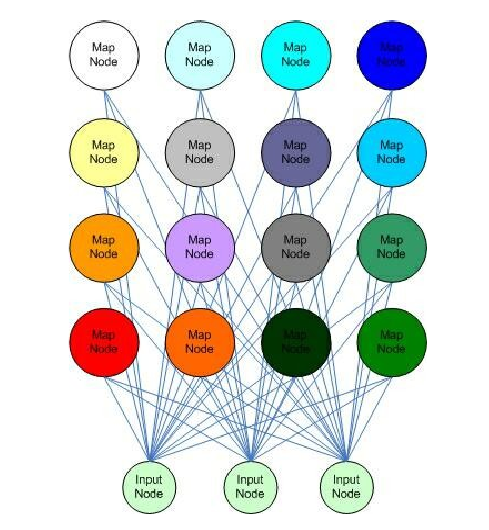
\includegraphics[width=1\textwidth]{img/node-som.png}
\label{fig:som-node}
\end{figure}

\subsection{Treinamento}\label{treinamento}
A rede SOM utiliza um algoritmo de aprendizado competitivo e não-supervisionado. para o aprendizado da rede. Um padrão de entrada é apresentado a rede, um neurônio vencem e inicia a atualização dos pesos do neurônio vencedor e de seus vizinhos (até um raio de vizinhança). Isto repete para cada nova entrada e a taxa de aprendizado e o raio de vizinhança são decrementados durante o processo.[Braga]

Atualização dos pesos do neurônio vencedor e de seus vizinhos:

\[ w_{ji}(t+1) = \left\{ 
  \begin{array}{l l}
    w_{ji}(t) + \eta(t)(x_{i}- w_{ji}(t)) & \quad \text{se j $\in$ $\Lambda$(t)}\\
    w_{ji}(t) & \quad \text{caso contrário}
  \end{array} \right.\]

Onde $w_{ji}$ é o peso entre os neurônios i e j, $\eta(t)$ é a taxa de aprendizado e $\Lambda$ é a vizinhança.

\begin{verbatim}
1:  Inicializar pesos e parâmetros;
2:  repita
3:     para todo padrão de treinamento faça
4:        Definir neurônio vencedor;
5:        Atualizar os pesos deste neurônio e de seus vizinhos;
6:        se o número do ciclo for múltiplo de N então
7:           Então reduzir a taxa de aprendizado;
8:        fim-se
9:     fim-para
10: até que mapa de características não mudar
\end{verbatim}

\subsection{Classificação de Cor}
Este é considerado o "Hello World" de SOMs. A maioria dos tutoriais publicados no
SOMs usam a classificação de cor SOM como seu principal exemplo. Isto é para uma muito
uma boa razão. Ao passar por este exemplo, o conceito de SOMs pode ser solidamente
apreendido. A razão pela qual a classificação de cor é bastante fácil de entender é por causa da
quantidade relativamente pequena de dados utilizados, bem como o aspecto visual dos
dados.

A classificação de cores do SOM usam apenas três pesos por mapa e nós de entrada.
Estes pesos representam a tripla (r, g, b) para a cor. Por exemplo, as cores podem
ser apresentado à rede, (1,0,0) para o vermelho (0,1,0) para o verde, etc A meta para
a rede aqui, é para aprender a representar todas essas cores de entrada em sua grade de duas dimensões,
mantendo as propriedades intrínsecas de tal como mantendo as
relações topológicas entre os vetores de entrada. Com isso em mente, se azul escuro
e azul claro são apresentados ao SOM, eles devem acabar ao lado do outro
da grelha de rede.

Para ilustrar o processo passo a passo através do algoritmo para a
aplicação de classificação da cor. O primeiro passo representa a inicialização da rede. A Figura \ref{fig:initial-node}
mostra uma rede recém inicializado. Cada quadrado representa um nó da rede.

\begin{figure}[ht]
\centering
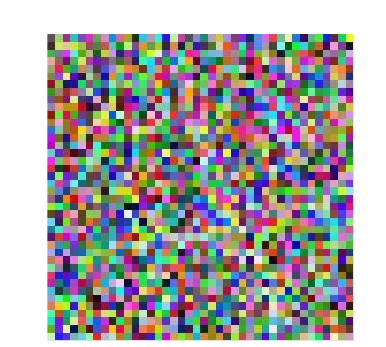
\includegraphics[width=0.7\textwidth]{img/initial-node.png}
\caption{Disposição inicial dos neurônios}
\label{fig:initial-node}
\end{figure}


O segundo passo é escolher um vetor de forma aleatória a partir dos vetores de entrada.
O passo 2 escolhe um vetor de forma aleatória a partir dos vectores de entrada. Oito vetores de entrada
são utilizados neste exemplo, que vão do vermelho para o amarelo para verde escuro. Em seguida,
o Passo 3 passa por cada nó e encontra BMU, conforme descrito anteriormente. A Figura \ref{fig:bmu-node}
mostra o BMU sendo selecionado na rede 4x4. A etapa 4 do
algoritmo calcula o raio vizinhança. Isto também é mostrado na Figura \ref{fig:bmu-node}. Todos
os nós em vermelho estão dentro do raio. No passo 5, em seguida, aplica-se o aprendizado
funções para todos estes nodos. Baseia-se na sua distância a partir do neurônio vencedor. O
neurônio vencedor (vermelho escuro) aprende mais, enquanto nós, na periferia do raio (luz
rosa) aprendem o mínimo. Nós fora do raio (branco) não aprendem nada.

\begin{figure}[ht]
\centering
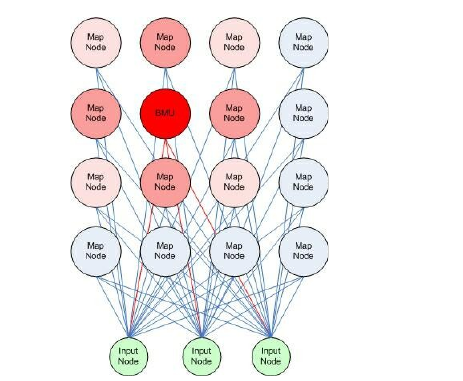
\includegraphics[width=0.7\textwidth]{img/node-bmu.png}
\caption{Nó vencedor}
\label{fig:bmu-node}
\end{figure}

Em seguida, volte para a Etapa 2 e repita. A Figura \ref{fig:final-node} mostra um SOM treinado,
representando todas as cores de oito entradas de cores. Observe como a luz verde fica ao lado do verde escuro,
e vermelho está ao lado de laranja.

\begin{figure}[ht]
\centering
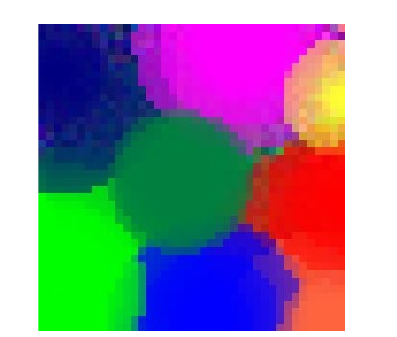
\includegraphics[width=0.7\textwidth]{img/final-node.png}
\caption{Estrutura do nó final}
\label{fig:final-node}
\end{figure}

\section{Métodos}\label{metodos}


\section{Resultados}\label{resultados}


\section{Conclusão}\label{conclusao}


\bibliographystyle{abbrv}
\bibliography{simple}

\end{document}